\section{Tension de surface}
\begin{figure}[ht]
	\centering
	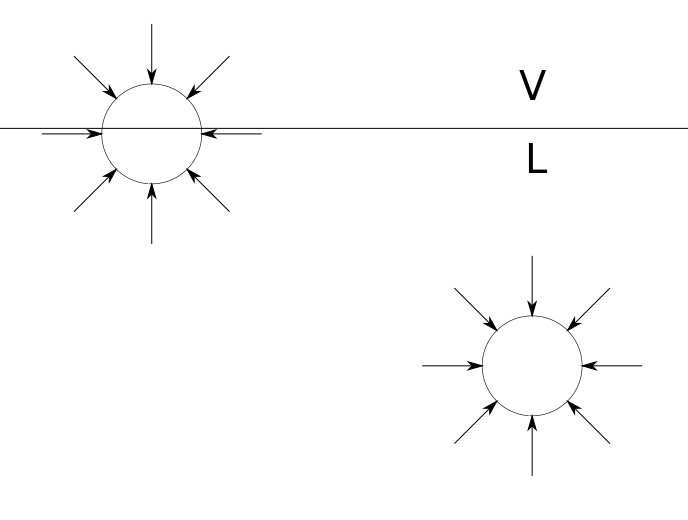
\includegraphics[scale = 0.3]{./image/rondforces.png}
	\caption{Ligne triple}
\end{figure}

La tension de surface est une force par unité de longueur.\\ 

Dans un liquide ayant une interface, une molécule complètement immergée dans le liquide est soumise à des forces d'interactions avec les autres molécules (du liquide) dans toutes les directions. 

Une molécule située à l'interface, la somme des interactions (avec les molécules du même fluide) est non nulle est dirigée vers l'intérieur du liquide. Il existe donc une force supplémentaire qui permet de maintenir l'interface.

Cette force supplémentaire (par unité de longueur) est la tension de surface.\\



la tension de surface est aussi une énergie par unité de surface, c'est l'énergie (par unité de surface) pour séparer les interfaces et les envoyer à l'infini l'une par rapport à l'autre.


\subsection{Mouillage}
Le mouillage est l'action de mouiller et mouiller consiste à  mettre en contact avec un liquide.\\


C'est le paramètre d'étalement $S = \gamma_{SV} - (\gamma_{SL} + \gamma_{LV}) = \gamma_{LV}(\cos\theta_{E} - 1)$ qui caractérise le mouillage lorsque la goutte est en équilibre sur un support matériel.

Quand $S > 0$, on parle de mouillage total et quand $S < 0$, on parle de mouillage partiel.\\

Nous nous intéressons en particulier à une goutte dont le support est une plaque plane dans les conditions de mouillage partiel. 
\begin{figure}[ht]
	\centering
	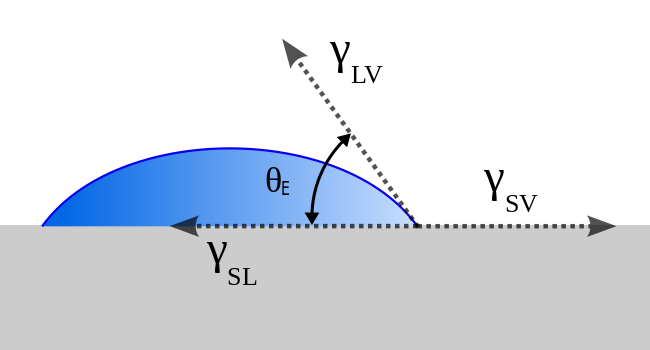
\includegraphics[scale = 0.3]{./image/Contact_angle2.png}
	\caption{Ligne triple}
\end{figure}



Le substrat est le nom donné au support (solide ou liquide) sur lequel la goutte de liquide repose.

Lorsqu'une goutte d'eau est posée sur support solide, il y a formation de 3 interfaces et donc de 3 tensions de surface.


En projetant les tensions de surface sur l'horizontale on obtient :

\begin{equation}
	\label{eq:Young}
	\gamma_{SV}  = \gamma_{SL} + \gamma_{LV}\cos\theta_{E}
\end{equation}

C'est la loi de Young.

\section{Hystérésis}


\begin{figure}[ht]
	\label{fig:hysteresis}
	\centering
	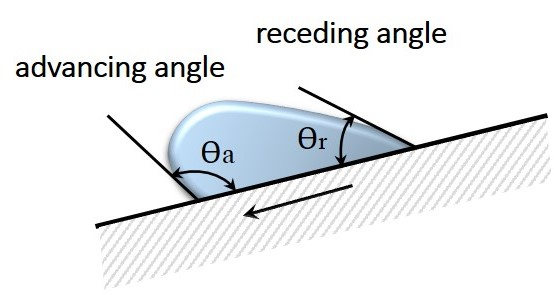
\includegraphics[scale = 0.8]{./image/hysteresis.jpg}
	\caption{Hystérésis}
\end{figure}
Dans la réalité l'angle statique $\theta_{E}$ n'est pas unique et on a :

\begin{equation}
	\theta_{R} <= \theta_{E} <= \theta_{A}
\end{equation}

Lorsque l'angle de contact $\theta$ vérifie $\theta < \theta_{R}$, la goutte se met à reculer et l'angle de contact $\theta$ à l'arrière de la goutte est appelé $\theta_{r}$.\\

Lorsque l'angle de contact $\theta$ vérifie $\theta > \theta_{A}$, la goutte se met à avancer et l'angle de contact $\theta$ à l'avant de la goutte est appelé $\theta_{a}$.\\

Dans le cas d'un surface parfaite $\theta_{a}$ et $\theta_{r}$ sont égaux.\\

L'hystéréris (en parlant d'angle de contact) est la différence $\theta_{a}-\theta_{r}$.

\section{Modèles d'angle dynamique}

L'angle de contact de la goutte en mouvement (l'angle dynamique) est différent de l'angle de contact quand la goutte es équilibre (angle statique).

Seuls des modèles existent pour estimer l'angle de contact dynamique et tous ses modèles se placent dans le cas d'une surface parfaite où on ne tient pas compte de l'hystérésis. 

Ces modèles font intervenir le nombre capillaire $C_{a}$, un longueur macroscopique $b$ et une longueur miscropique $a$.
\begin{equation}
	C_{a} 
	= \frac{\text{effets visqueux}}{\text{effets capillaires}} 
	= \frac{\eta U}{\gamma}
\end{equation}
\subsection*{Modèle De Gennes} 

\begin{equation}
	\label{modele:gennes}
	\theta 
	\left(\theta^{2} - \theta_{s}^{2}\right) 
	= \pm 6\ln\left(\frac{b}{a}\right)C_{a}
\end{equation}
\subsection*{Modèle Cox et Voinov}  

\begin{equation}
	\label{modele:Cox}
	\theta^{3} - \theta_{s}^{3} = 
	\pm 
	9\ln\left(
	\frac{b}{a}\right) C_{a}
\end{equation}
\subsection*{Modèle de cinétique moléculaire}  

\begin{equation}
	\left(\theta^{2} - \theta_{s}^{2}\right) 
	\propto C_{a}
\end{equation}
\subsection*{Modèle linéaire} 

\begin{equation}
	\theta - \theta_{s} \propto \pm U
\end{equation}

